\documentclass{article}
% Packages
\usepackage[a4paper, total={15cm, 24cm}, bmargin=28mm, footskip=15mm]{geometry}
\usepackage[T1]{fontenc}
\usepackage[utf8]{inputenc}
\usepackage{amsmath}
\usepackage{amssymb}
\usepackage[mediumspace, squaren]{SIunits}
\usepackage{verbatim}
\usepackage{hyperref}
%\usepackage{parskip} %skip the indent of a new paragraph.
\usepackage{booktabs} 
\usepackage{float}
\usepackage{graphicx}
\usepackage{caption}
\usepackage{multirow}
\usepackage{epstopdf}
\graphicspath{ {figures/} }
\usepackage{import}
\usepackage{url}
\usepackage{todonotes}
\usepackage{subfig}
\usepackage{parskip}
\usepackage{blindtext}
{\setlength\intextsep{0pt}}
\newcommand{\squeezup}{\vspace{-2.5mm}}
\newcommand*\NewPage{\newpage\null\thispagestyle{empty}\newpage}
\usepackage{ucs}
\usepackage{xcolor}

% Information about document
\author{Ignacio Scibona & \& & Helene Hogstad Fossum}
\date{April 2018}
\title{TMR4290 - Project 2: \\ Design of a Marine Electric Power System}

\begin{document}

% Titlepage 
\begin{titlepage} 
    \maketitle
    \thispagestyle{empty}
    \begin{figure}
    \centering
    
\includegraphics[width=0.5\textwidth]{utils/logontnu_eng.pdf}
    \end{figure}
    
\end{titlepage}

% Table of Contents (not sure if we need)
% \newpage
% \pagenumbering{Roman}

% \tableofcontents

% Main report (NB! Use input files)
\pagenumbering{arabic}
\setcounter{page}{1}
\newpage
\section{Introduction}

\subsection{Main Characteristics}

\begin{itemize}
    \item Propulsion Type: VSI-type VSD propulsion units %VSD: Variable Speed Drive - VSI Voltage Source Inverter
    \item Propulsion Power: 42 MW
    \item Drilling Power: 23 MW
    \item Emergency Propulsion Power 34 MW
    \item Emergency (single failure) Service Load: 4MW
    \item Thruster Drives Type: 12-pulse single type, 
    \item Drilling Drives Type: Multidrive two separate feeders type with 12-pulse rectifiers.
    \item Distribution Voltage: 3 $ \times $ 400 V
    \item Distribution Power Factor: 0.9
\end{itemize}


 
\newpage
\section*{Problem 1}

\subsection*{1a)} \label{problem_1a}


According to the "Activities Regulations" of the Petroleum Safety Authority Norway \cite{Petroleum_Authority}, Chapter XVI, Re Section 90, Table 1, drilling and well activities where well control is ensured by a facility with dynamic positioning, the required equipment class is to be 3. As the semi-submersible is to be classed by DNV GL, the required class would be DYNPOS(AUTRO) which is their class 3 DP-system class \cite{RulesShipsDNVGLPart6Chap3}. \todo{done?}

\begin{comment}

\cite{Petroleum_Authority}

Chapter XVI - Maritime Operations
Section 90 - Positioning
Table 1 Equipment Class

d) Drilling and well activities: Where well control is ensured by a facility with dynamic positioning: Class 3

The equipment class is described in the IMO/MSC Circular 645, Chapter 2, Equipment Classes.

2.9 Functional requirements
In order to meet the single failure criteria it will normally be necessary to provide:
1) For equipment class 2 - redundancy of all active components.

2) For equipment class 3 - redundancy of all components and physical separation of the components.
\end{comment}

\section*{Problem 2}
\subsection*{2a)}

In order to fulfill the Equipment Class 3 required by the Petroleum Safety Authority Norway (as specified in \nameref{problem_1a}) and in accordance to the DNV GL regulations \ref{Sec:Equivalent_Notations} \cite{RecommendedPractices_DP_DNVGL}, the notation will be DYNPOS(AUTRO). The tables in appendix \ref{Sec:Equipment_Requirements} and \ref{Sec:Class_Notations} specifies the DNV GL requirements for each part of the system that is needed to be classed as DYNPOS(AUTRO). 

To summarize, there should be redundancy in all active components and there should be physical separation of compartments. The system must be designed such that the vessel is able to maintain it's position long enough to safely terminate the work in progress after a single failure. This would correspond to for example ending a drilling operation in our case. There should be enough remaining thrust and power to maintain position after a worst-case failure. The system must also be designed such that minimum operator interference is required to switch on redundant equipment and this equipment should be available immediately \cite{RulesShipsDNVGLPart6Chap3}.
\todo{This is all from the same source and the same as in the table. Everything is just rephrased like in question 3. Not sure if this is ok.}


%Such notation sets as a design requirements:

% \begin{itemize}
%     \item Redundancy of all active components (classification societies interpret this differently).
%     \item Physical separation of the components.
%     \item Time to terminate: Be able to maintain station long enough to safely terminate the work in progress after a \textit{single failure}.
%     \item The equipment intended to provide redundancy is available immediately and with a minimum of operator intervention.
%     \item Adequate remaining power and thrust after a \textit{worst-case failure}
% \end{itemize}

%%%% OLD %%%
% In order to fulfill the Equipment Class 3 required by the Petroleum Safety Authority Norway (as specified in \nameref{problem_1a}) and in accordance to the DNV GL regulations \ref{Sec:Equivalent_Notations} \cite{RecommendedPractices_DP_DNVGL}, the notation will be DYNPOS(AUTRO). The tables in appendix \ref{Sec:Equipment_Requirements} and \ref{Sec:Class_Notations} specifies the DNV GL requirements for each part of the system that is needed to be classed as DYNPOS(AUTRO). 

% Such notation sets as a design requirements:

% \begin{itemize}
%     \item Redundancy of all active components (classification societies interpret this differently).
%     \item Physical separation of the components.
%     \item Time to terminate: Be able to maintain station long enough to safely terminate the work in progress after a \textit{single failure}.
%     \item The equipment intended to provide redundancy is available immediately and with a minimum of operator intervention.
%     \item Adequate remaining power and thrust after a \textit{worst-case failure}
% \end{itemize}

% \todo[inline]{Keep reading recommended practices from page 22}

\section*{Problem 3}
\subsection*{3a)}
% DP System
\myParagraph{DP system:} \label{par:Def_DP_system}

DNV GL defines a \textit{DP vessel} (dynamically positioned vessel) as a vessel that is capable of automatically maintain its position and heading either along in a fixed position or along a predetermined path. As opposed to i.e thruster assisted mooring, this has to happen by only using thruster force\cite{RulesShipsDNVGLPart6Chap3}. 

DNV GL then defines a \textit{DP system} as consisting of a \textit{power system}, a \textit{thruster system}, a \textit{DP-Control system} and an \textit{independent joystick system} \cite{RulesShipsDNVGLPart6Chap3}. The power- and thruster systems are explained in Section \nameref{sec:3b}. 

The \textit{DP-Control system} is defined as all control systems, hardware and software that is used by the vessel to be a DP vessel. This includes \textit{sensor systems}, displays, operational panels, a \textit{positioning reference system}, one or more \textit{uninterruptble power supply(s) (UPSs)}, the needed cabling and the dynamic positioning control computer(s) \cite{RulesShipsDNVGLPart6Chap3}.  
\todo{Do we also have to explain sensor system, UPS and positioning reference system?}

The \textit{Joystick system} provides manual control of the system, letting the operator define the output thrust, including turning moment \cite{RulesShipsDNVGLPart6Chap3}. \todo{Add for which classes of DP systems the joystick is required} 

% Consequence analysis
\myParagraph{Consequence analysis:}
\textbf{Consequence analysis} is defined by DNV GL as a system a part of the DP-control system that issues an alarm if the vessel is unable to be in DP operate under the current weather conditions if the worst case failures occurs. These requirements are set in advance \cite{RulesShipsDNVGLPart6Chap3}. 


%%%%%%%%%%%%%%%%%% 3b) %%%%%%%%%55%%%%%%%%%%%
\subsection*{3b)} \label{sec:3b}
\myParagraph{Power system:}
DNV GL defines the \textbf{Power system} as all components and systems necessary to supply the DP system with power. That would include the prime movers with auxiliary systems, the generators, the switchboards, the UPSs, the cabling and distribution system. If the system is classed as DYNPOS(AUTR) or DYNPOS(AUTRO), it also includes a power management system (PMS) \cite{RulesShipsDNVGLPart6Chap3}.  


\myParagraph{Thruster system:}
DNV GL defines the \textbf{Thruster system} as all components necessary to supply the DP system with thrust force and direction. That would include the thrusters with drives including the auxiliary system, the thruster control system, the necessary cabling and the main propellers and rudders if they are also part of the DP system \cite{RulesShipsDNVGLPart6Chap3}. (The main propellers and/or thrusters can be disconnected from the DP system and only used in transit. In that case, the DP system would only consist of tunnel thrusters, azimuth thrusters etc.)




%%%%%%% 3c) %%%%%%%%%%%
\subsection*{3c)}

\myParagraph{Reliability:} 
In the DNV GL rules, \textbf{Reliability} ability of a component or system to perform its required function without failure during a specified time interval

\myParagraph{Redundancy:} 
\textbf{Redundancy} is defined as the ability of a component or system to maintain its function when one failure has occurred.
Classification societies interpret \textit{redundancy} differently. For DNV GL it can be achieved, for instance, by installation of multiple components, systems or alternative means of performing a function \cite{RulesShipsDNVGLPart6Chap3}. It should also take into account the long term loss of a major item of machinery such as a generator or thruster \cite{RecommendedPractices_DP_DNVGL}. \todo{Add another definition by another classification society to see the difference?}

\todo[inline]{By now it is copy-paste}

\myParagraph{Redundancy Group:} 

all components and systems that is subject to a single failure as specified in [4], for the specific notations

Guidance note:
The redundancy groups will emerge as a consequence of the worst case single failure within each
group. The rules do not give requirements to the number of (beyond 2) or ratio between the
defined groups. The groups should be identified in the FMEA, verified by testing and incorporated in
the consequence analysis

    \begin{comment}
    \cite{RecommendedPractices_DP_DNVGL} page 26.
    
    There are three key elements in any redundancy concept:
    1) performance
    2) protection
    3) detection
    
    THEN THEY EXPLAIN EACH. SEE IF WE NEED TO INCLUDE THIS
    \end{comment}

%%%%%%% 3d) %%%%%%%%%%%
\subsection*{3d)} \label{Sec:3d}

\myParagraph{Failure}: 
DNV GL defines \textbf{failure} as an occurrence in a component or system causing one or both of the following effects:
\begin{itemize}
    \item loss of component or system function.
    \item deterioration o f functional capability to such an extent that the safety of the vessel, personnel or environment is significantly reduced.
\end{itemize}

Depending on the DP class, the definition of single failure includes or not certain failure modes. For DYNPOS(AUTRO) it includes: incidents of fire and flooding and all break-downs of systems and components.

\myParagraph{Worst-case failure}: failure that results in the largest reduction of the position and/or heading keeping capacity. This means loss of the most significant redundancy group, for the prevailing operation.

\todo[inline]{6.11 Consequence analysis
6.11.1 The dynamic positioning control systems shall perform an analysis of the ability to maintain position after worst case failures. An alarm shall be initiated, with a maximum delay of 5 minutes, when a failure will cause loss of position in the prevailing weather conditions. In case the redundancy is based on limited energy sources like e.g. batteries then the duration of the delay should be considered.
Guidance note:
This analysis should verify that the thrusters and generators remaining in operation after the worst case failure can generate the same resultant thruster force and moment as required before the failure.}
\section*{Problem 4}
\section*{Problem 5}
\section*{Problem 6}
\newpage
\section*{Problem 7}
This problem is largely explained in section \nameref{prob_5and6}, but on a different format. Without repeating a lot of the same arguments, the system should be able to deliver enough propulsion, drilling and service power as described in the task description under normal operation. In the case of single failure, it must be able to deliver the minimum propulsion and service load power. This is achieved with having redundant generation groups and two thrusters in each corner. Loosing one (or two) generation group will not lead to too little generated power. Loosing one (or two) thruster groups will not lead to too little propulsion power. This is summed up in Tables \ref{tab:redundantDesignIntention} and \ref{tab:AND_OR_redundantDesignIntention} designed on the same form as in \cite{RedundantDesignIntention_DNV}. \todo{Is this okay? It seem to be OK ;p}

% As stated before, DNV GL defines worst-case failure as the single failure that causes the loss of the most significant redundancy group. In this design, that would correspond to losing one segregation. However, the system was designed to be more redundant and able to withstand losing more than one subsection.  


\begin{table}[h]
    %\centering
    \begin{tabular}{|l|l|l|}
        \hline
        \text{Redundancy design intention} & & \\
        \hline
        \makecell{\text{Normal operation \\ before failure} $\rightarrow$} & \makecell{\text{3 OR 4 generation groups are \\ running. In total, able to \\ provide 66MW} as calculated in table \ref{tab:powerDemand}} & \makecell{\text{Active redundancy \\ from redundant \\ generation groups}}\\
        \hline
        \makecell{\text{In the case of \\ a single failure} $\rightarrow$} & \makecell{\text{3 OR 2 generators groups are running. \\ In total, able to provide \\ 38MW as calculated in table \ref{tab:powerDemand}}} &  \makecell{\text{Active redundancy \\ from redundant \\ generation groups}}   \\
        \hline
    \end{tabular}
    \caption{Redundancy design intention explained}
    \label{tab:redundantDesignIntention}
\end{table}

\begin{table}[h]
    %\centering
    \begin{tabular}{|l|l|l|}
        \hline
        \text{Redundancy design intention} & & \\
        \hline
        \makecell{\text{Normal operation \\ before failure} $\rightarrow$} & \makecell{(G1 AND G2 AND G3) \\ OR (G1 AND G3 AND G4) \\ OR (G1 AND G2 AND G4) \\ OR (G2 AND G3 AND G4) \\ OR (G1 AND G2 AND G3 AND G4)} & \makecell{\text{Active redundancy \\ from redundant \\ generation groups}}\\
        \hline
        \makecell{\text{In the case of \\ a single failure} $\rightarrow$} & \makecell{(G1 AND G2 AND G3) \\  OR (G1 AND G3 AND G4) \\ OR (G1 AND G2 AND G4) \\ OR (G2 AND G3 AND G4) \\OR (G1 AND G2) OR (G1 AND G3) \\ OR (G1 AND G4) OR (G2 AND G3) \\ OR (G2 AND G4) OR (G3 AND G4)} & \makecell{\text{Active redundancy \\ from redundant \\ generation groups}}   \\
        \hline
    \end{tabular}
    \caption{Redundancy design intention}
    \label{tab:AND_OR_redundantDesignIntention}
\end{table}

\begin{table}[h]
    \centering
    \begin{tabular}{|l|l|l|}
    \hline
    \multicolumn{3}{|c|}{\textbf{Redundancy design intention overview by redundant and common component groups}} \\
    \hline
    \text{Redundant A groups} & \text{Common X groups} & \text{Redundant B groups} \\
    \hline
    
    \end{tabular}
    \caption{Redundant and common component groups}
    \label{tab:RedundantComponentGroups}
\end{table}
\section*{Problem 8}
The genset that has been used as reference in the design is the MAK Marine WM 46 DF described in \cite[p.128 -129]{CatGenerators}. There it states that the generator efficiency is approximately 0.96\% and the power factor is 0.8. A power factor value of 0.8 is also assumed in the NORSOK standard \cite{NORSOKstandard}, therefore these values are adopted for the calculations. 

\subsection*{8a)}
The voltage adopted for the main switchboards is 11kV, that is the recommended level by the NORSOK standard \cite[p.10]{NORSOKstandard} for systems where the total installed generated power exceeds 20MW.

In the design used, the thrusters are also connected to separate switchboards. For such power levels, the NORSOK standard recommends voltage levels between 2.4 and 6.6kV \cite{NORSOKstandard}. The adoption of such voltages would lead to the need of installing one transformer on each feeder, which would lead to significant extra cost and a more complex design. It was therefore decided to keep the voltage level at 11kV also for these switchboards. %\todo{Confirm with the lecturer/TA if this is OK}  

% Regarding the Thrusters' switchboards, the standards recommend voltage levels between 2.4 and 6.6 kV. But the adoption of such voltages would lead to the installation of one transformer on each feeder, then it has been decided to keep the 11kV level on the switchboards.

%It was decided that the main switchboards should have a voltage level of 11kV. This was decided after first calculating the total power demand in the system and then using the IF

% \todo{Remember to ask and clarify the voltage level of the thrusters' switchboards}

\subsection*{8b)}

%\todo{Ask if the transformers should work at a partial load (i.e if their rating should be more than 4MWe)}

\todo[inline]{Helene v2:}
The service load after single failure (assumed the same for worst case failure) is 4MW and the service load under normal operations is in Section \nameref{Sec:designRequirements} assumed to be 12MW. It is required, that each distribution transformer shall be capable of feeding all the low voltage consumers in two redundant subsections simultaneously. In this design, the worst-case failure condition is defined as two generator groups out of service, meaning two transformers are out of service. 

Under normal operation, the four transformers should therefore be able to supply a minimum of 12MWe power combined. In this design, the transformers are chosen to be 4MW each, making it possible to supply sufficient power with three transformers and one in stand-by. 

For worst-case failure condition, the two remaining transformers should be able to provide 4MWe power each. Using the power factor of 0.9, the rated power for the distribution transformers would be 

\[
Power\, Rating=\frac{4MWe}{0.9}=\underline{4444\,kVA}
\]

\todo[inline]{Old?}

% Old
% Since the service load after single failure is 4MW, and each distribution transformer shall be capable of feeding all the low voltage consumers in two redundant subsections simultaneously (given requirements) and the defined \textit{worst case failure} is taken as two subsection out of service, each of them should be capable of supplying 4MW active power. 
% %\todo{ask if here should we comment something about the reactive power with the 0.9 power factor given}.

% Other requirement to take into account is the service load during normal operation, which is not given and has been assumed to be 12MW for the calculations.

% Finally, the transformers should be capable of supplying at least 4MWe active power each and 12MWe combined. 4MWe has been adopted as the rated power for each of the service load transformers, thus being capable of supplying each of them the \textit{worst case failure} service load and the normal operation service load combined with other two, leaving one in stand-by condition. Finally, the rated power for the distribution transformers, assuming a power factor value of 0.9, would be:

% \[
% Power\, Rating=\frac{4MWe}{0.9}=\underline{4444\,kVA}
% \]

%\todo[inline]{I don't exactly understand what do they mean with 'Each distribution transformer shall be capable of feeding all the low voltage consumers in two redundant subsections simultaneously'

%\todo[inline]{What we need the power factor for?}

\subsection*{8c)}

A proper \textit{maximum continuous rating} (MCR) for gensets is one that makes the gensets work in an appropriate load condition. That is, between 70 and 90\% of the load.  
%\todo{check percentages with TA} in all conditions.

For the adopted gensets configuration and the power requirements for normal and \textit{worst case failure} conditions, and a MCR of 14MWe for the gensets (17500 kVA for a power factor value of 0.8 \cite{CatGenerators}) will allow the gensets to work at 71.98\% or 83.98\% load when 7 or 6 gensets are connected respectively. 

In the same way, for \textit{worst case failure} if 4 gensets were connected, they would work at 72,96\% load or, in extreme case, 3 gensets could supply the required power at 97.28\% load. A MCR between 12.5kWe and 14.5 kWe (15625 and 18125 kVA at 0.8 power factor) would allow the gensets to work in good load conditions. 

The reference values for the efficiency is 96\% and power factor is 0.8 \cite{CatGenerators}. Assuming this, a proper MCR for the diesel engine would be
\[
MCR_{engine}=\frac{17500 \, kV\!A \times 0.8}{0.96}=14583 \, kW
\]

%\todo[inline]{power factor is not given for the thrusters. Should we work with 0,8? or only with active power?}

\subsection*{8d)}

%\todo[inline]{should we calculate complex or only real current? we don't have power factors}

The 3-phase current through the generator breakers assuming a power factor of 0.8 power factor is

\[
P=3\,V\,I\,cos(\phi) \Rightarrow I_{RMS}=\frac{14000 \, kW\!e}{3 \times 11 kV \times 0.8}=530.30 A \Rightarrow I_{Peak}=\sqrt{2}\,I_{RMS}=750\,A
\]

\subsection*{8e)}

%\todo[inline]{power factor and working load for the thrusters' transformers?}

Since the given propulsion power requirement is 42 MW for the worst environmental condition and 34 MW for the \textit{worst case failure} condition, a suitable MCR for the thrusters' motors can be 6.3 MW (the maximum available in the market nowadays is 6.5 MW). With such rating, the propulsion requirement can be supplied by 8 thrusters at 83.3\% load in the worst environmental condition and by 6 at 90\% load in the \textit{worst case failure} condition. 

% Helene: 
Assuming a power factor of 0.9 and the same efficiencies for the transformer, motor and frequency converter as in table \ref{tab:efficiencies}, a suitable rating for the transformer can be

% For supplying 6.3 MWe power, a suitable rating for the transformer can be, assuming the values for its power factor 0.9 and 0.993 efficiency, and 0.960 and 0.985 for the motor and frequency converter efficiencies respectively as stated in Table \ref{tab:efficiencies}:

\[
S_{t}=\frac{6.3\,MW}{cos(\phi)\,\eta_t\,\eta_f\,\eta_m}=\frac{6300\,W}{0.9 \times 0.993 \times 0.985 \times 0.960}=7455 \, kV\!A
\]


\subsection*{8f)}

%\todo[inline]{only active power? or complex?}

The total required power for \textit{worst case failure} condition is, as shown in Table \ref{tab:powerDemand}, 40.86MW, and since the in such condition there will be foru 14MW generators available: 

\[
Remaining\,\,Power=4 \times 14\,MWe - 40.86\,MWe = 56\,MWe - 40.86\,MWe = \underline{15.14 \, MWe}
\]



% References
\newpage
\thispagestyle{empty}
\bibliographystyle{IEEEtran}
\bibliography{bibliography.bib}


% Appendix
\newpage
\pagenumbering{Alph}
\setcounter{page}{1}
\section*{Appendix}\label{Appendix}
\appendix
\renewcommand{\thesubsection}{\Alph{subsection}}

%%%%%%%% DP Class %%%%%%%%%
\subsection{DP Class Requirements}\label{Sec:DP_Class_Requirements} 

\subsubsection{Equipment requirements}\label{Sec:Equipment_Requirements}
\begin{figure}[h]
    \centering
    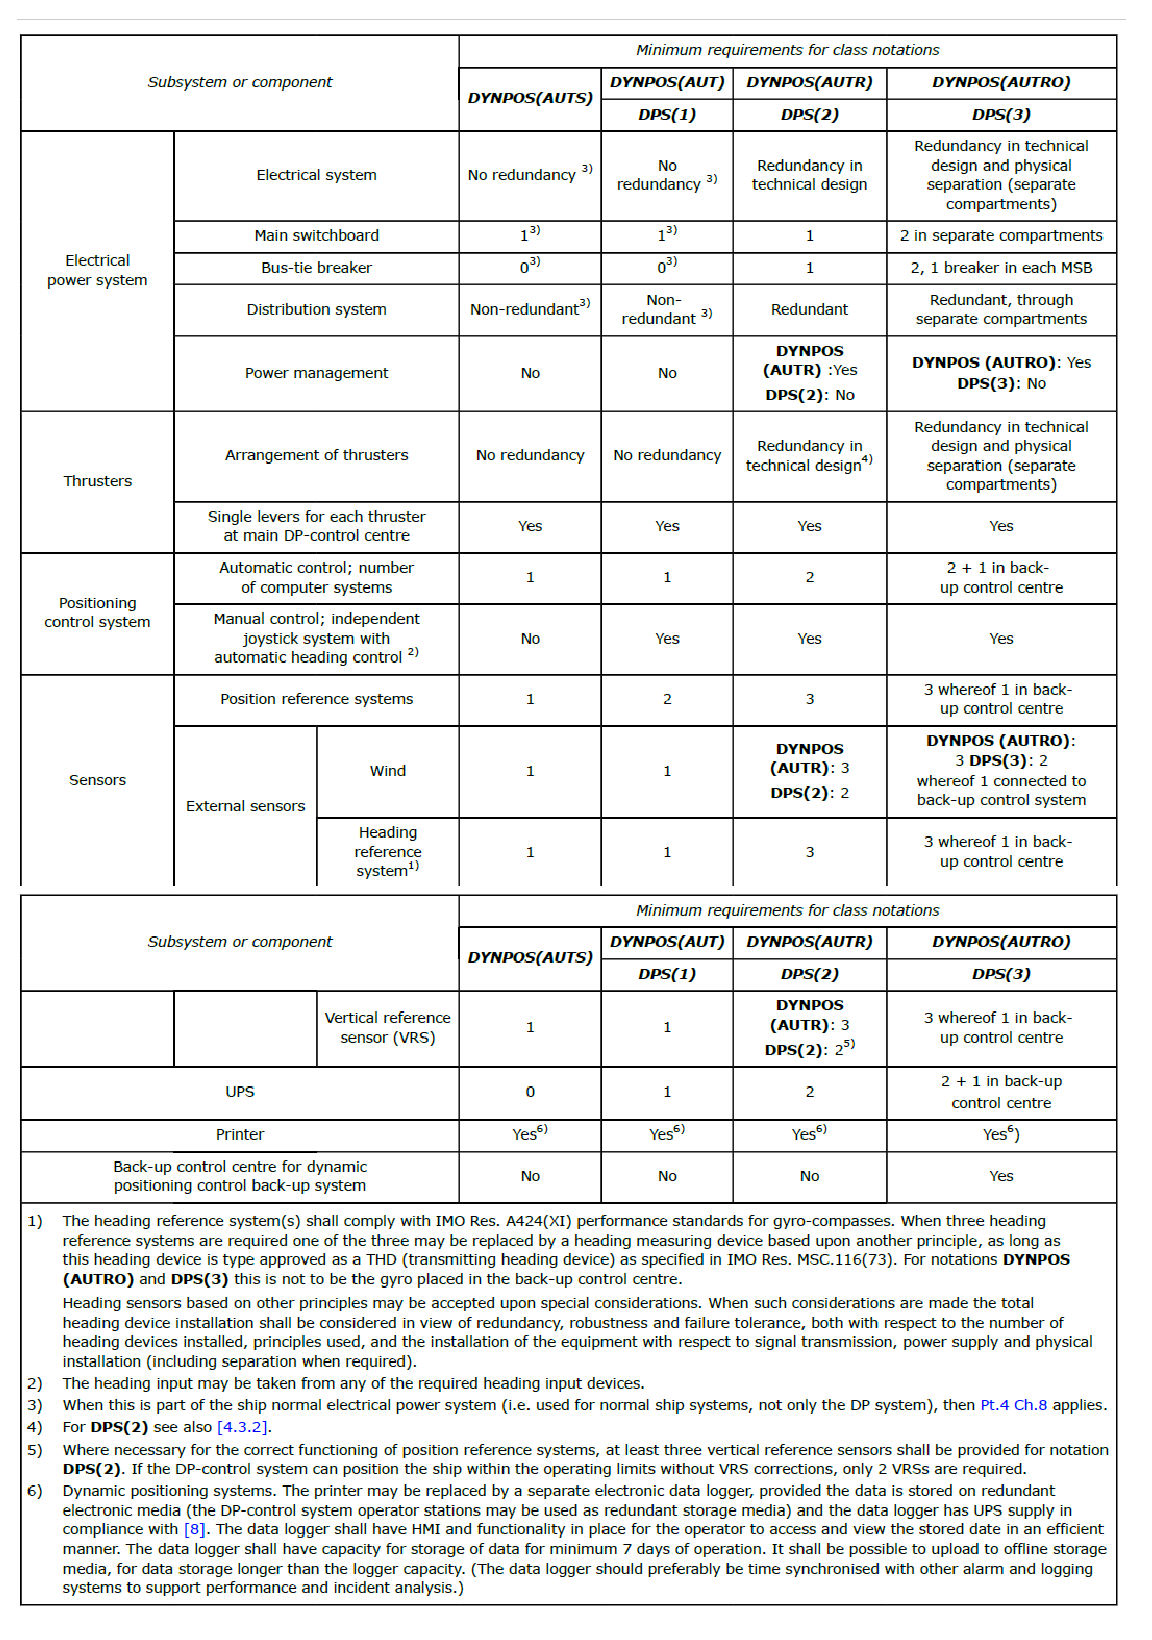
\includegraphics[width = 0.95\textwidth, height = 0.73\textheight]{figures/DP_requirements_table.eps}
    \captionof{table}{Minimum requirements for equipment on DP vessels for the different classifications \cite{DNV-GL_RP_Dynamic_positioning} .}
\end{figure}

\newpage
\subsubsection{Class Notations}\label{Sec:Class_Notations} 
\begin{figure}[h]
    \centering
    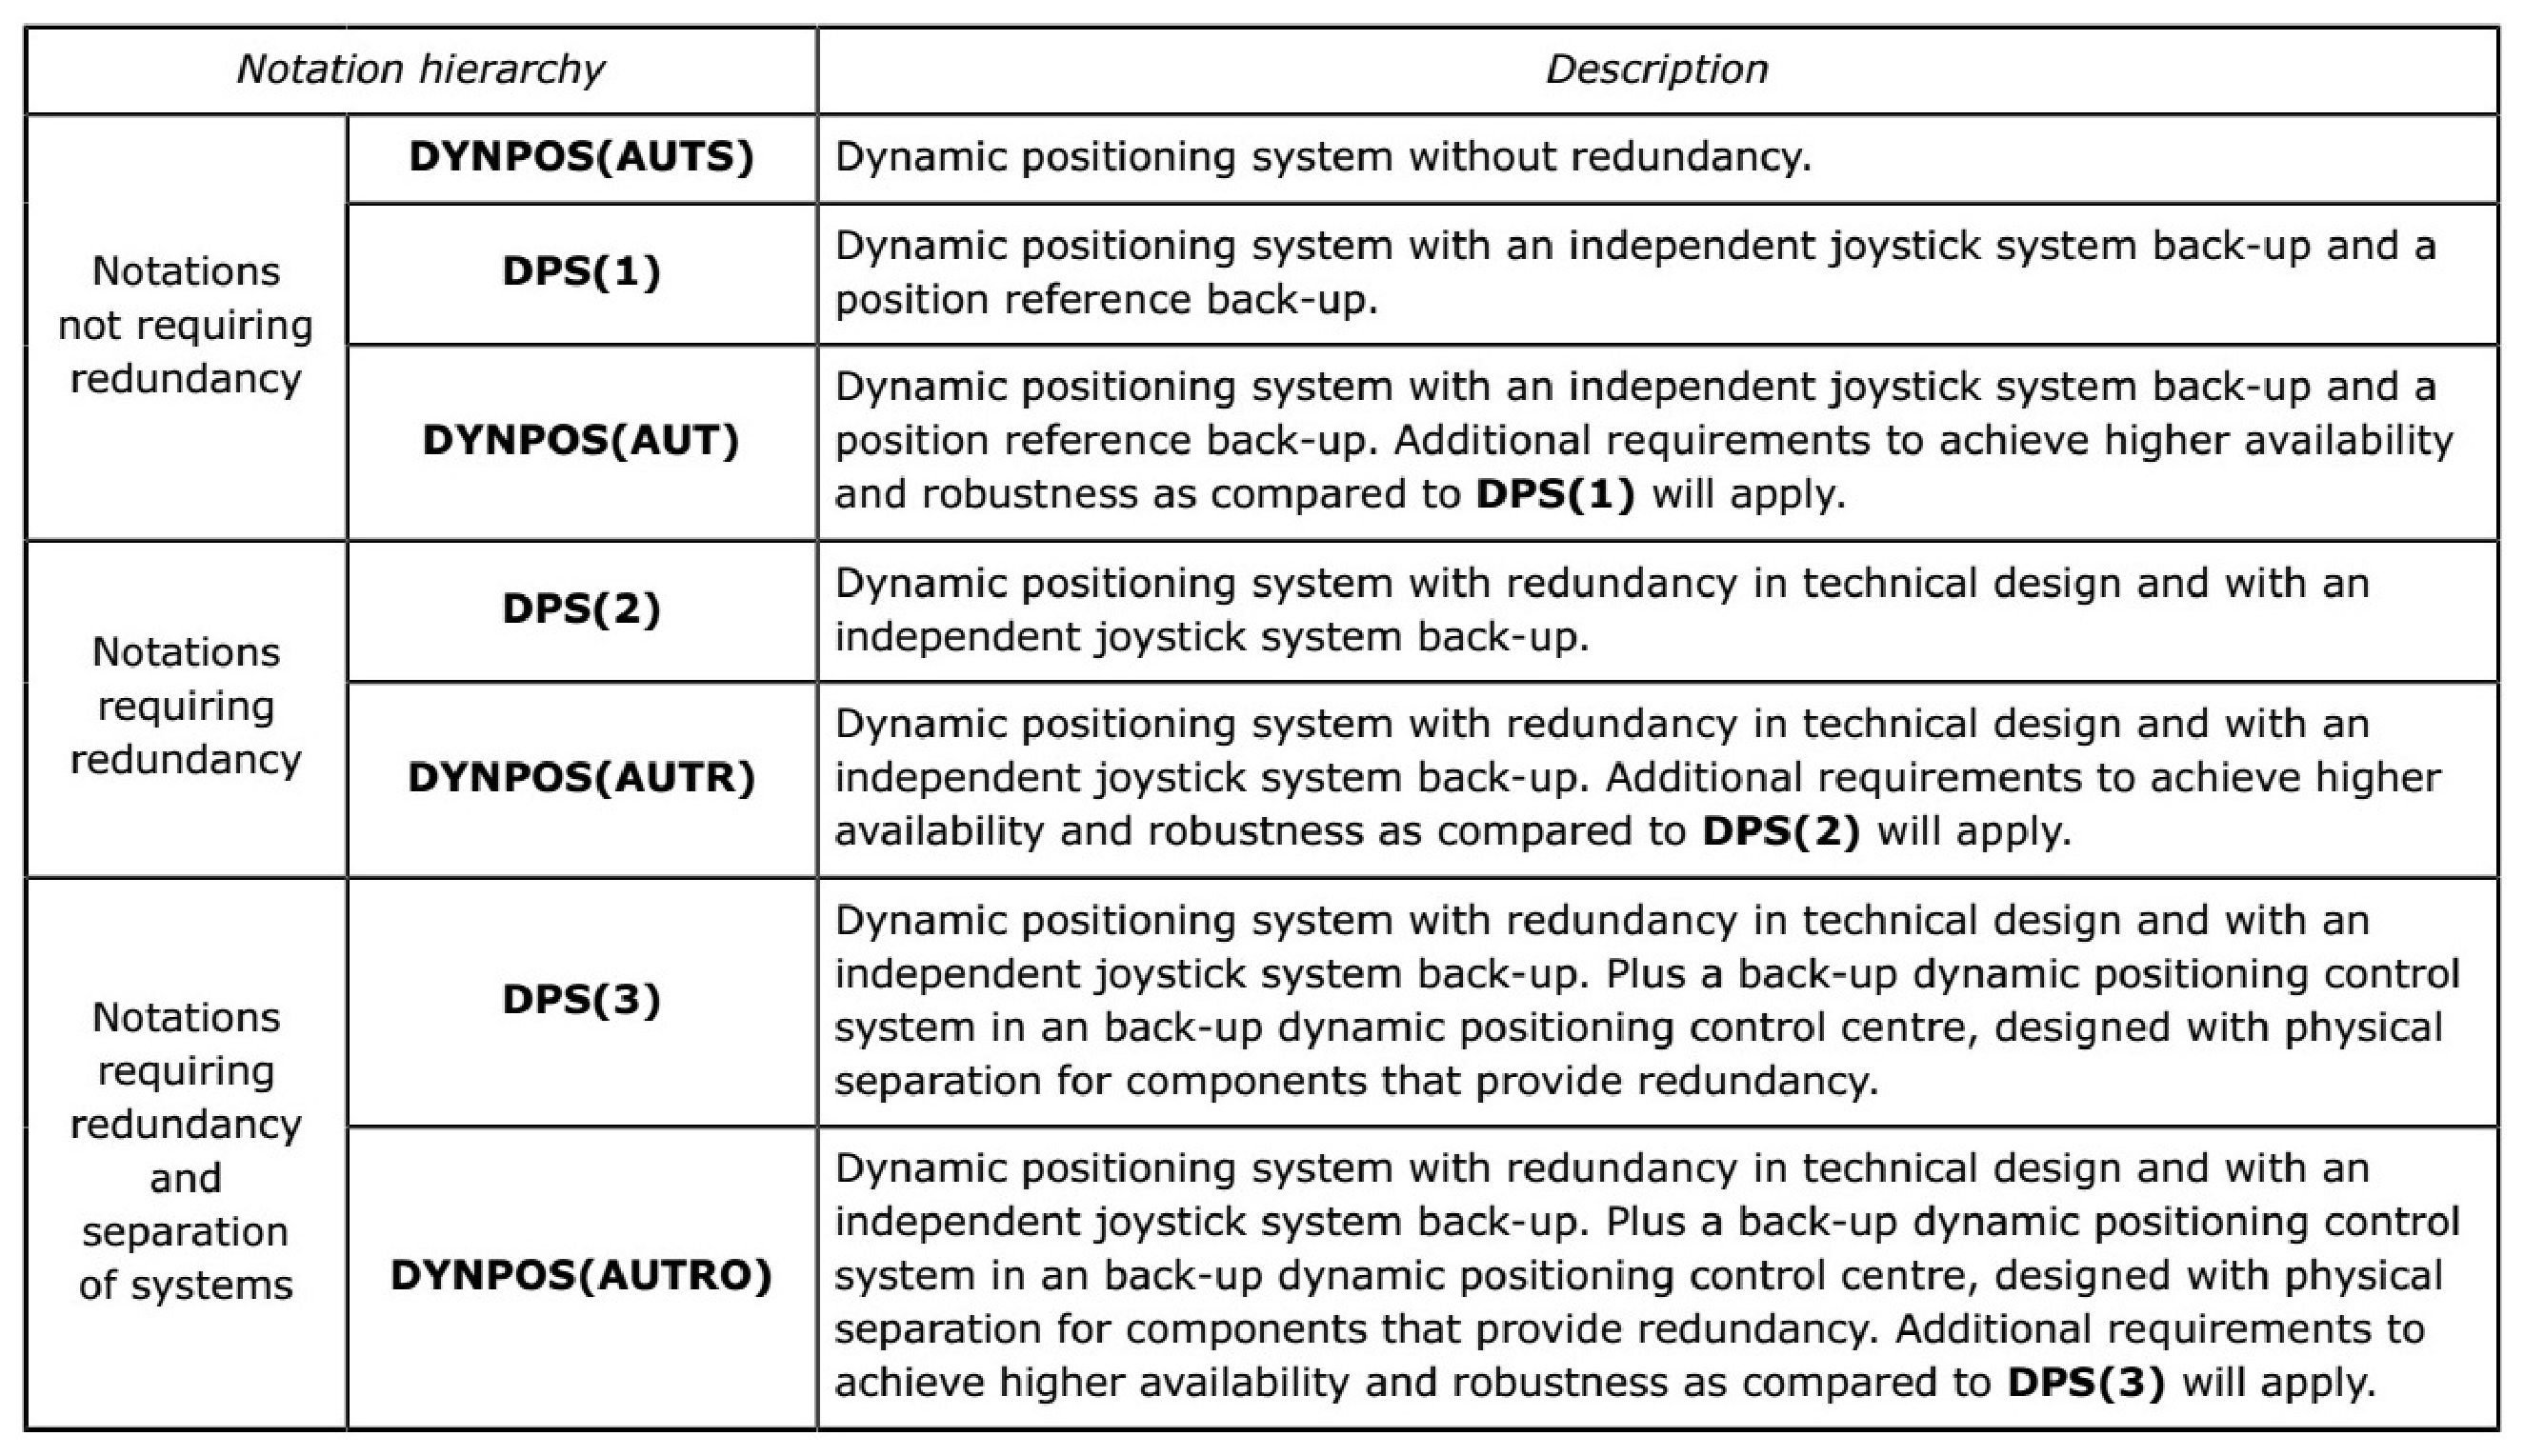
\includegraphics[width = \textwidth]{figures/DP_Class_notations.eps}
    \captionof{table}{Dynamic Positioning Class Notations. \cite{DNV-GL_Regulations_ship}}
\end{figure}

\subsubsection{DP Class Equivalent Notations}\label{Sec:Equivalent_Notations} 
\begin{figure}[h]
    \centering
    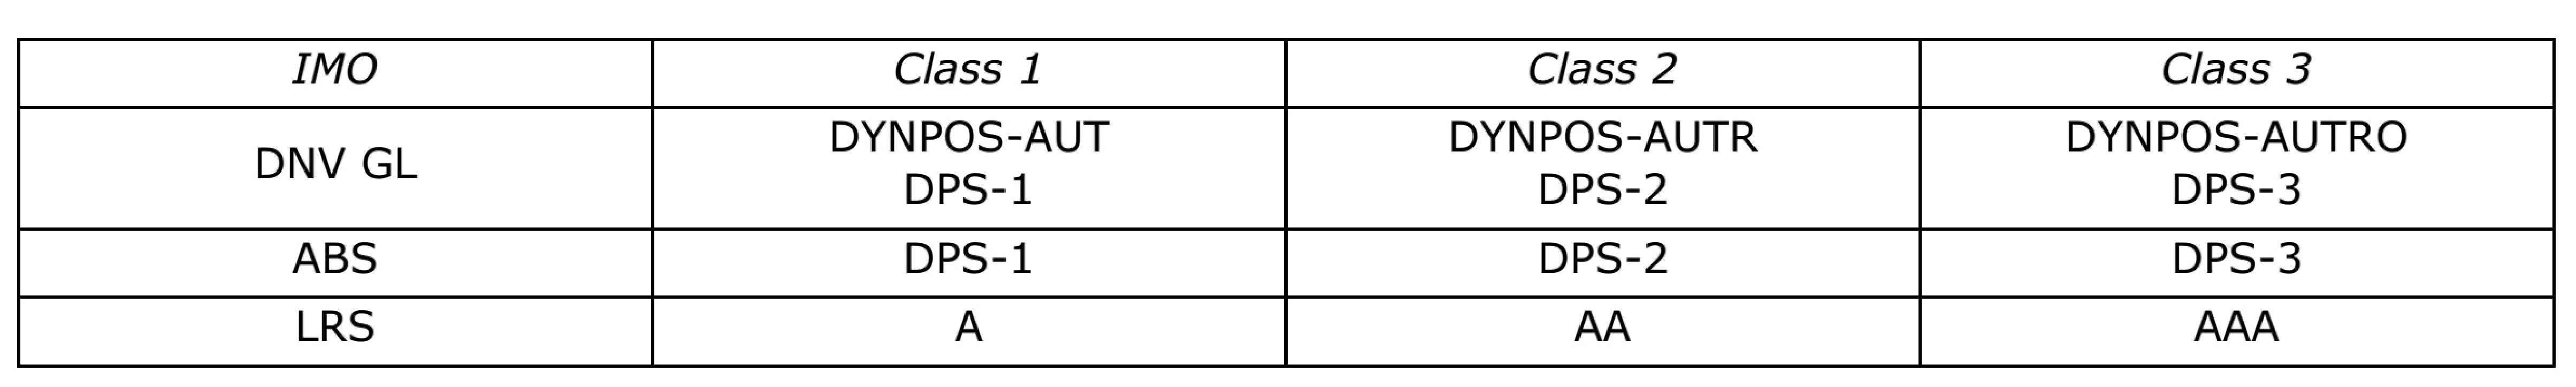
\includegraphics[width = \textwidth]{figures/DP_Class_equivalent_notations.eps}
    \captionof{table}{Class Equivalent Notations \cite[page.22]{DNV-GL_RP_Dynamic_positioning}}
\end{figure}



\end{document}
